\section{Appendix}
Below two plots showing the by the trackpy library found centre of masses of the beads are displayed. These plots indicate the tightening of the axes for increased laser output.
\subsection{Particle Spread}
\begin{figure}[!ht]
    \centering
    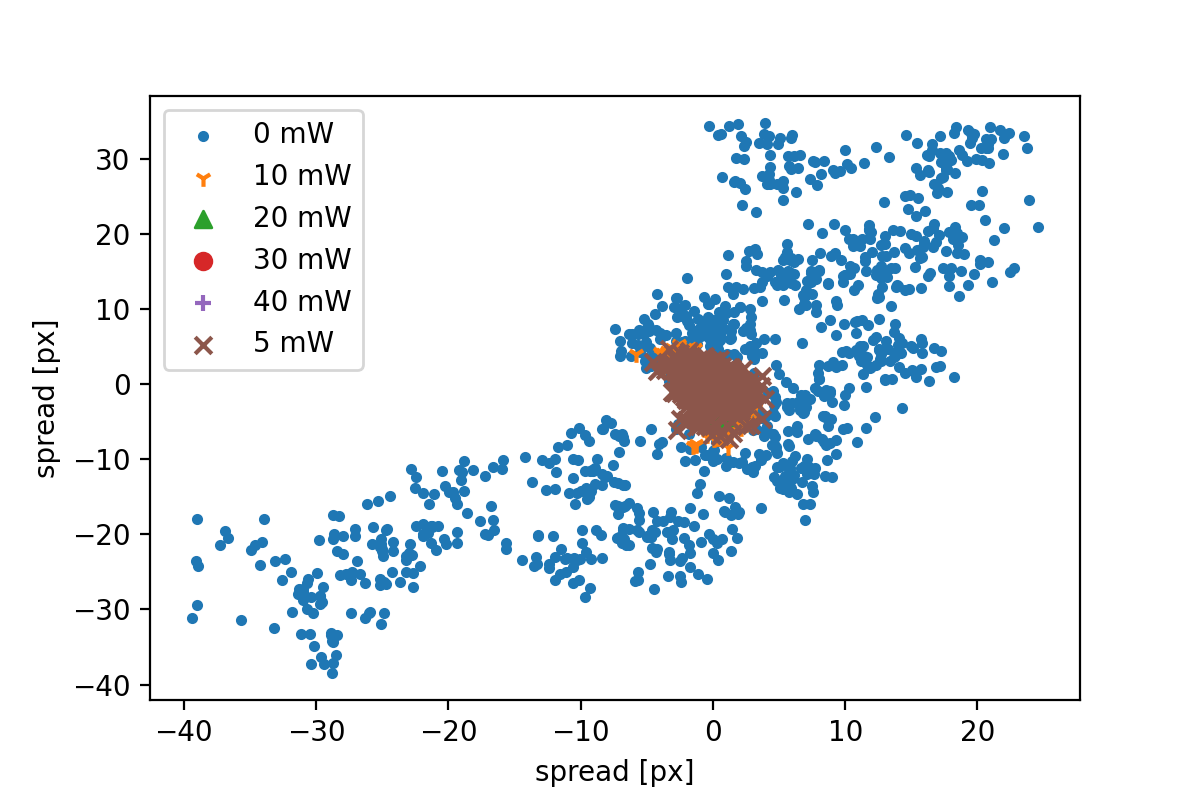
\includegraphics[width=.8\textwidth,keepaspectratio]{figures/spread-dataset1.png}
    \caption{Spread of the first dataset shifted towards origin by average displacement from centre}
\end{figure}
\begin{figure}[!ht]
    \centering
    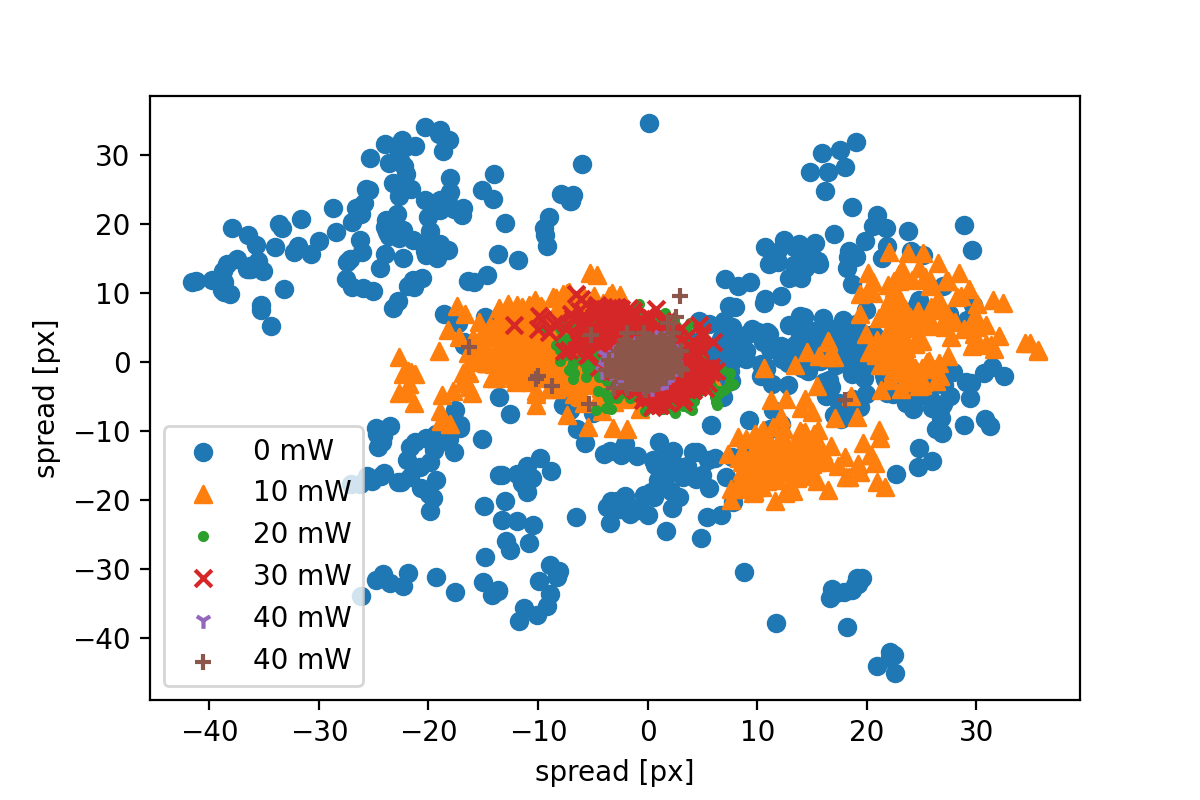
\includegraphics[width=0.8\textwidth,keepaspectratio]{figures/spread-dataset2.png}
    \caption{Spread of the second dataset shifted towards origin by average displacement from centre}
\end{figure}
\clearpage
\subsection{Python}
The python code used to calculate the ellipse axes is displayed below.
\begin{lstlisting}[language=Python]
def ellipse_calc(x,y):
    # replace nans by average
    x_ = np.where(np.isnan(x), np.nanmean(x), x)
    y_ = np.where(np.isnan(y), np.nanmean(y), y)

    # Calculate variance and covariance
    var_x = np.sum((x_-np.mean(x_))**2)/(len(x)+1)
    var_y = np.sum((y_-np.mean(y_))**2)/(len(y)+1)
    cov = np.sum((x_-np.mean(x_))*(y_-np.mean(y_))/(len(x_)+1))

    cov_matrix = np.asarray([[var_x, cov],[cov,var_y]])
    evals,evecs = linalg.eig(cov_matrix)
    evecs_ = evals*evecs
    #plt.plot(x,y, linestyle='none',marker='x',zorder=1)
    #plt.quiver(np.nanmean(x),np.nanmean(y), -evecs_[1,:],-evecs_[0,:],zorder=2, units='xy', scale=1, width=1e-8, headwidth=4)


    a = np.max(evals)
    b = np.min(evals)
    print(a)
    print(b)
    index_a = np.where(evals == a)[0]
    theta = np.arctan(evecs[0,index_a]/evecs[1,index_a])
    print('theta =', theta)
    return a,b,theta
\end{lstlisting}



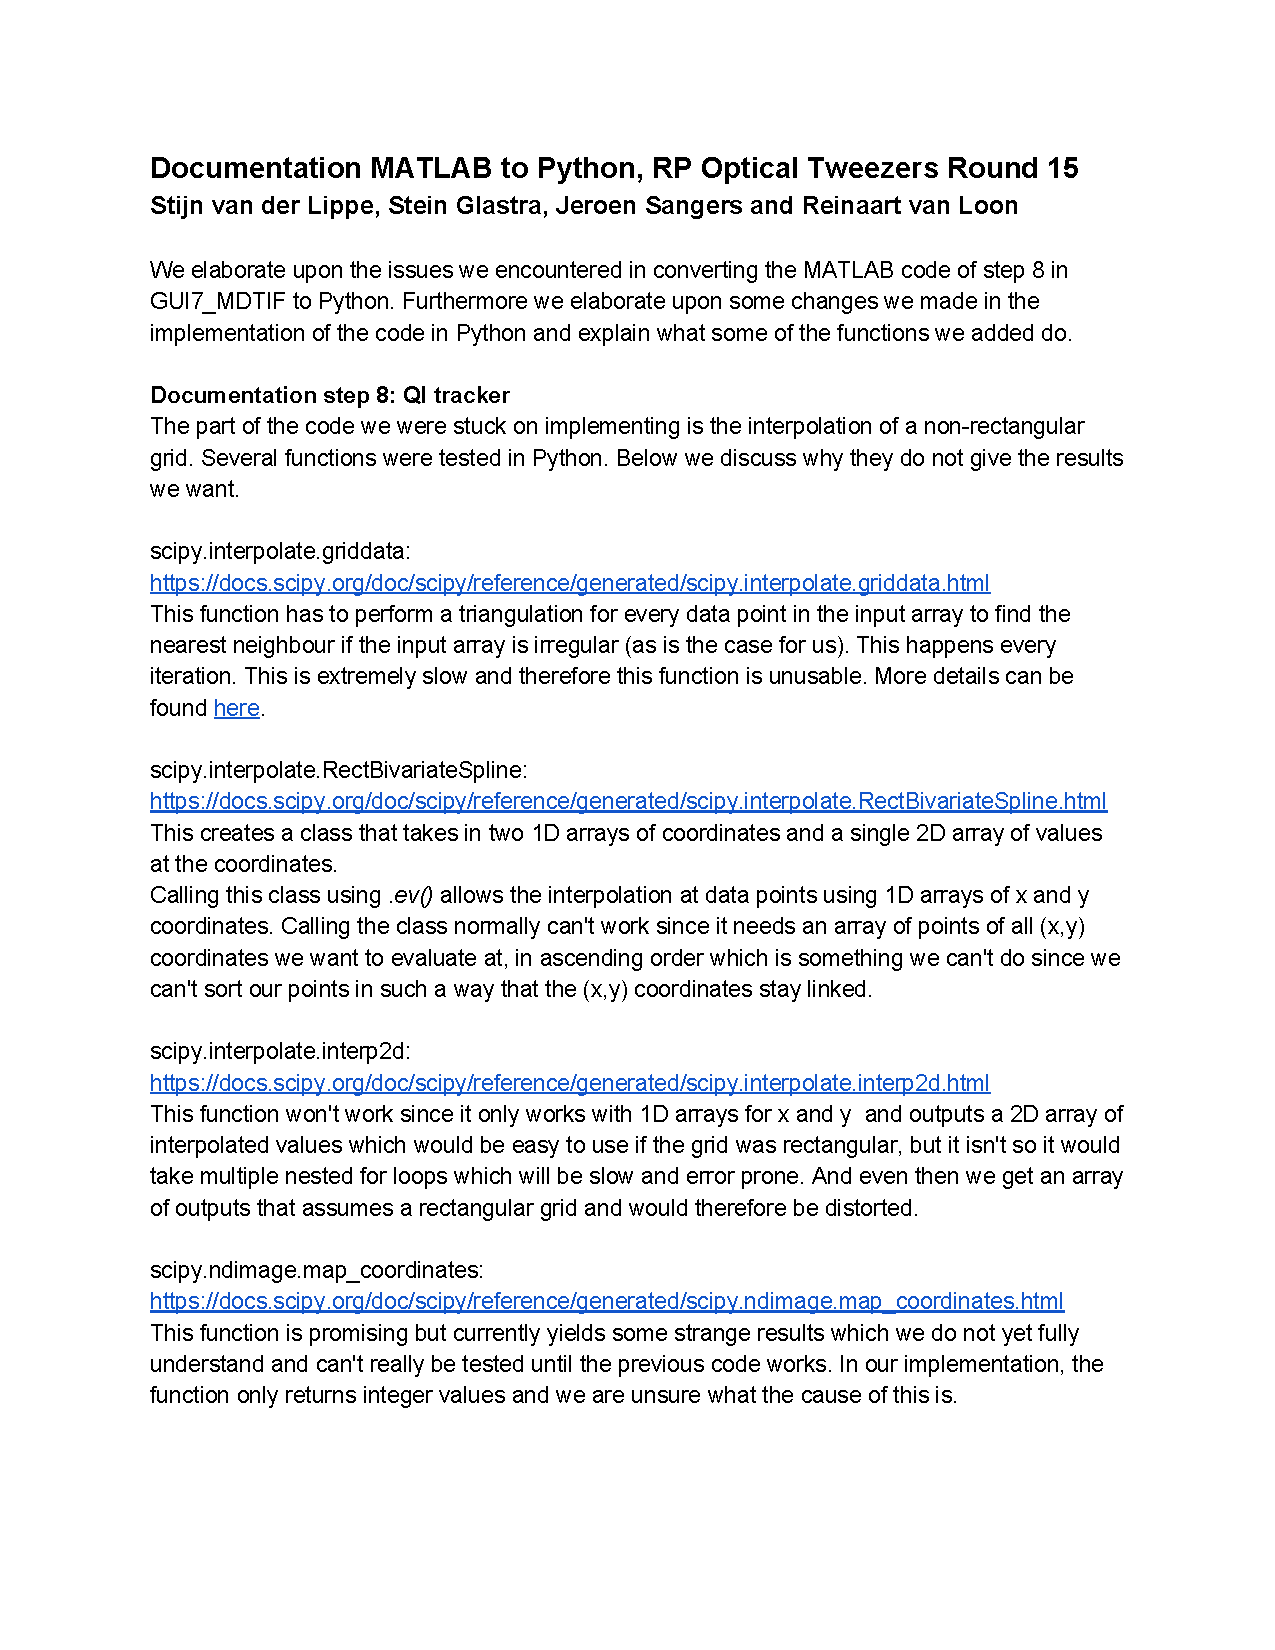
\includepdf[pages=-]{python_algorithmes_uitleg.pdf}








